\documentclass{article}
\begin{document}
\section{header 1}
test words

\subsection{Test Case 7: Wide Tree Structure}
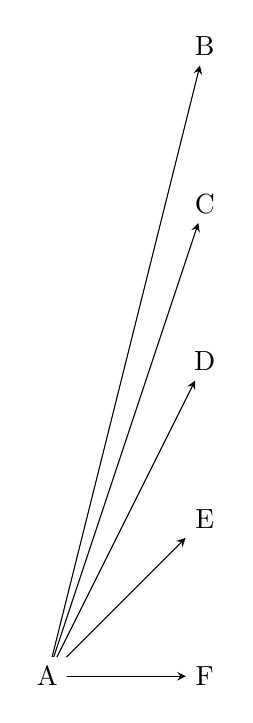
\begin{tikzpicture}[>=stealth]
\node (A) at (0, 2) {A};
\node (B) at (2, 10) {B};
\node (C) at (2, 8) {C};
\node (D) at (2, 6) {D};
\node (E) at (2, 4) {E};
\node (F) at (2, 2) {F};
\draw[->] (A) -- (B);
\draw[->] (A) -- (C);
\draw[->] (A) -- (D);
\draw[->] (A) -- (E);
\draw[->] (A) -- (F);
\end{tikzpicture}
same paragraph

\end{document}
